\begin{exercise}
\begin{figure}[H]
\centering
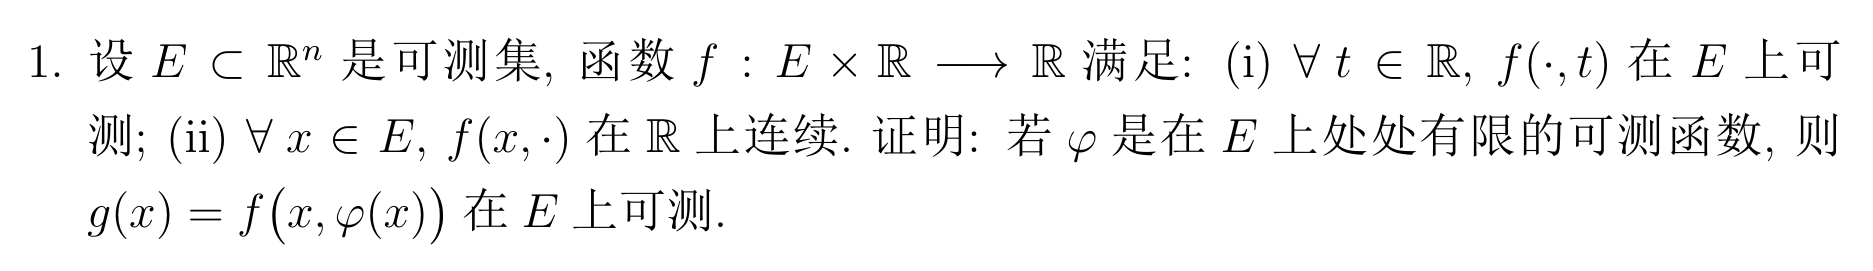
\includegraphics[width=\textwidth]{1-hw8-2025042920.png}
% \caption{}
\label{}
\end{figure}
\end{exercise}
\begin{proof}
Denote $f_{x}\coloneqq f(x,\cdot)$, $f_{t}\coloneqq f(\cdot,t)$. Then for any open set $\mathcal{O}\subset \mathbb{R}$
\[
\begin{aligned}
g^{-1}(\mathcal{O}) & =\{ x\in E:g(x)\in \mathcal{O} \} \\
 & =\{ (x,\varphi(x))\in E\times \mathbb{R}:f(x,\varphi(x))\in \mathcal{O} \}  \\
 & =\bigcup_{x\in E}(x,\overbrace{ \varphi ^{-1}(\underbrace{ f_{x}^{-1}(\mathcal{O}) }_{ \text{open} }) }^{ \in \mathcal{M}_{\mathbb{R}} }) \\
 & \in \mathcal{M}_{\mathbb{R}^{n+1}}
\end{aligned}
\]
\end{proof}

\begin{exercise}
\begin{figure}[H]
\centering
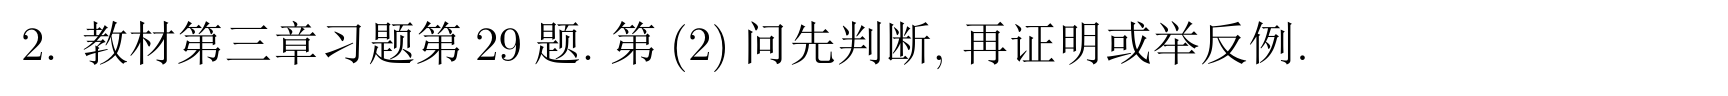
\includegraphics[width=\textwidth]{2-hw8-2025042920.png}
% \caption{}
\label{}
\end{figure}
\begin{figure}[H]
\centering
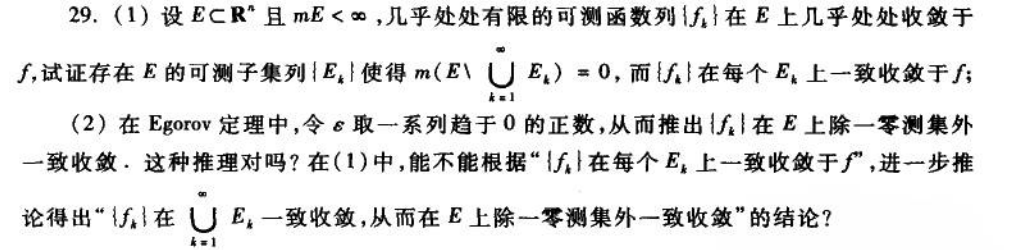
\includegraphics[width=\textwidth]{3-hw8-2025042920.png}
% \caption{}
\label{}
\end{figure}
\end{exercise}
(1)

\begin{theorem}[Egoroff's Theorem]
Assume $E$ has finite measure. Let $\{f_n\}$ be a sequence of measurable functions on $E$ that converges pointwise on $E$ to the real-valued function $f$. Then for each $\epsilon>0$, there is a closed set $F$ contained in $E$ for which
\[
\{f_n\} \rightarrow f \text { uniformly on } F \text { and } m(E \sim F)<\epsilon .
\]
\end{theorem}
By Egoroff's theorem, for each $k$, there exists closed $E_k\subset E$ s.t.
\[
\{ f_n \}\to f\text{ uniformly on }E_k\text{ and }m(E\setminus E_k)<\frac{1}{2^{k}}
\]
Thus
\[
\begin{aligned}
m\left( E\setminus \bigcup_{k=1}^{\infty} E_k \right) & =m\left( E\cap\left( \bigcup_{k=1}^{\infty} E_k \right)^{c} \right)=m\left( E\cap \left( \bigcap_{k=1}^{\infty} E_k^{c} \right) \right) \\
 & =m\left( \bigcap_{k=1}^{\infty} (E\cap E_k^{c}) \right)=m\left( \bigcap_{k=1}^{\infty} (E\setminus E_k) \right) \\
 & \leq m(E\setminus E_k)<\frac{1}{2^{k}}\qquad \forall k\geq 1
\end{aligned}
\]
Let $k\to \infty$ then
\[
m\left( E\setminus \bigcup_{k=1}^{\infty} E_k \right)=0
\]
(2) The reasoning is wrong.

\begin{figure}[H]
\centering
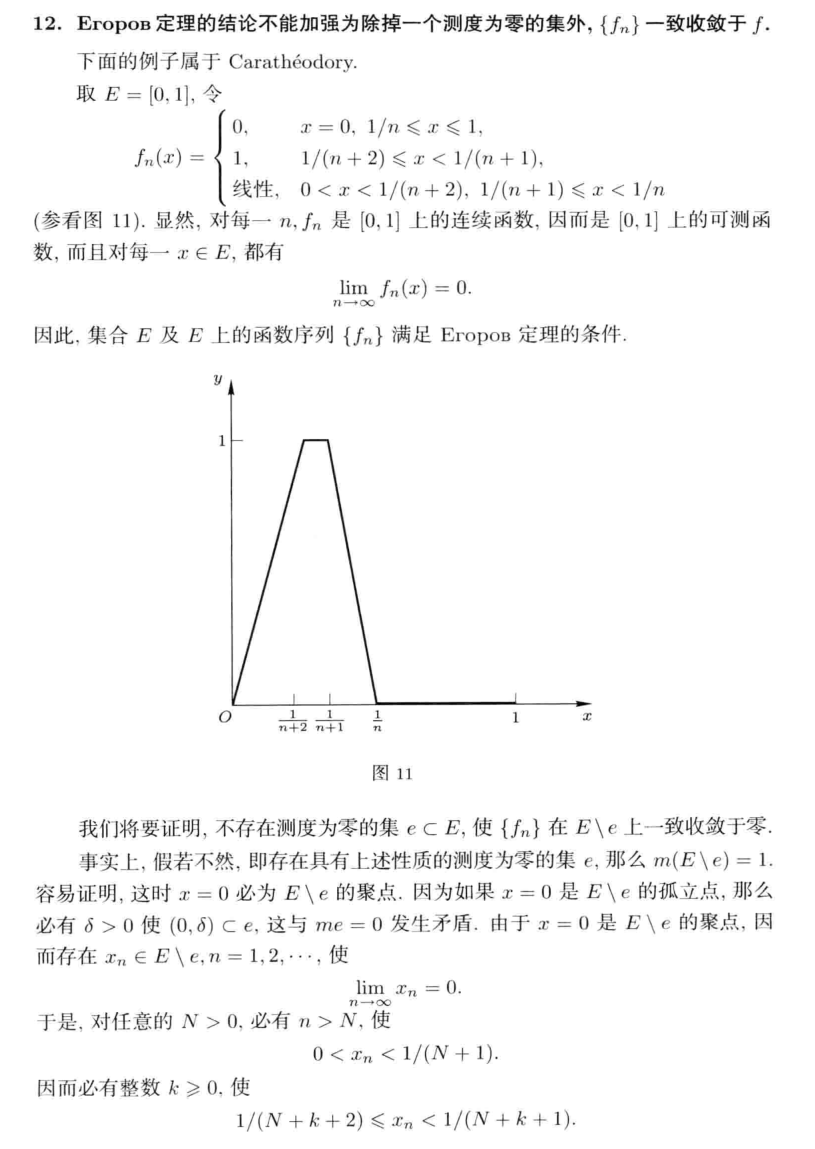
\includegraphics[width=\textwidth]{hw8-2025042923.png}
% \caption{}
\label{}
\end{figure}
\begin{figure}[H]
\centering
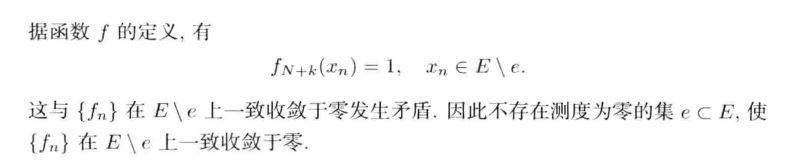
\includegraphics[width=\textwidth]{1-hw8-2025042923.png}
% \caption{}
\label{}
\end{figure}

\begin{exercise}
\begin{figure}[H]
\centering
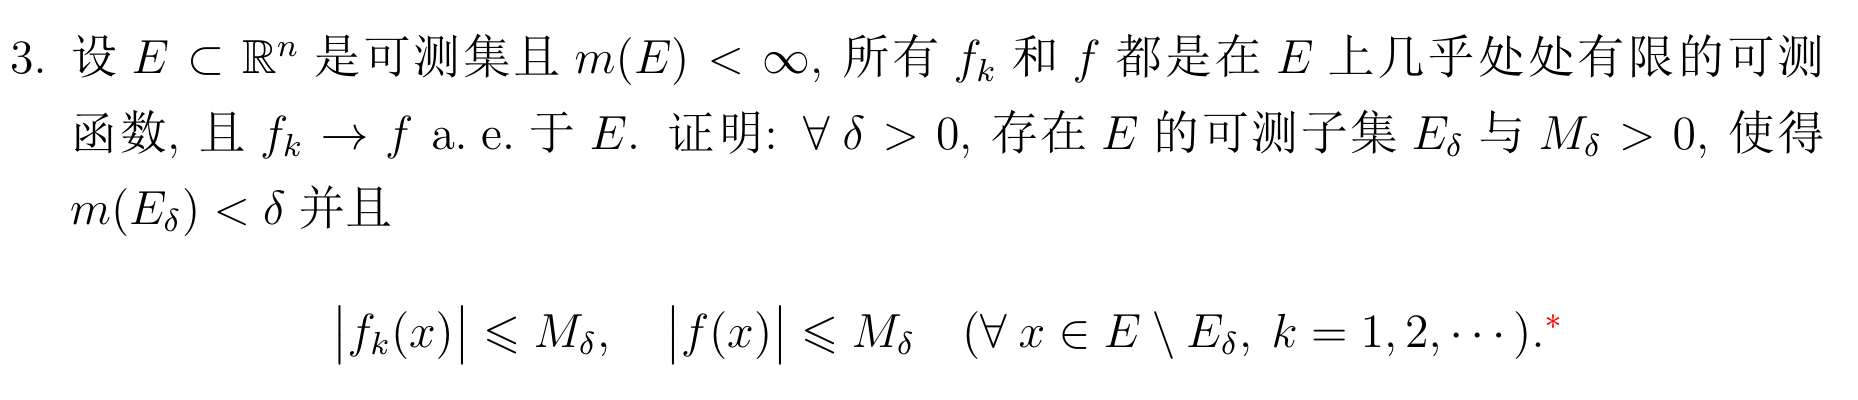
\includegraphics[width=\textwidth]{4-hw8-2025042920.png}
% \caption{}
\label{}
\end{figure}
\end{exercise}
Let $E_0=\{ f_k\not\to f \}\cup \{ f=\pm \infty \}$, then $mE_0=0$. Apply Egoroff's theorem to $E\setminus E_0$, for any $\delta>0$, there exists $F\subset E\setminus E_0$ s.t.
\[
f_n\to f\text{ uniformly on }F\text{ and }m((E\setminus E_0)\setminus F)<\delta/3
\]
There exists $K>0$ s.t.
\[
\sup_{x\in F}\lvert f_k(x)-f(x) \rvert <1\qquad \forall k\geq K
\]
Since $f_k$ is finite a.e. on $E$, there exists $E_k\subset E$ s.t.
\[
\sup_{x\in E_k}\lvert f_k \rvert \leq M_k \text{ and }m(E\setminus E_k)<\delta/(3K-3)
\]
And
\[
\sup_{x\in \bigcup_{k=1}^{K-1}E_k }\lvert f_k-f \rvert \leq \max_{1\leq k\leq K-1}M_k\text{ and }m\left( E\setminus \bigcup_{k=1}^{K-1} E_k \right)<\delta/3
\]
There exists $\widetilde{E}\subset E$ s.t.
\[
\sup_{x\in \widetilde{E}}\lvert f \rvert \leq M\text{ and }m(E\setminus \widetilde{E})<\delta/3
\]
Therefore
\[
\sup_{x\in \left( \bigcup_{k=1}^{K-1} E_k \right)\cup\widetilde{E}}\lvert f_k \rvert \leq M+\max_{1\leq k\leq K-1}M_k+1\qquad \forall k\geq 1
\]
where $m\left( E\setminus \left( \left( \bigcup_{k=1}^{K-1} E_k \right)\cup\widetilde{E} \right) \right)<2\delta/3$. Define
\[
E_{\delta}=F\setminus\left( \left( \bigcup_{k=1}^{K-1} E_k \right)\cup \widetilde{E} \right),\quad M_{\delta}=M+\max_{1\leq k\leq K-1}M_k+1
\]
Then
\[
m(E_{\delta})\leq m(E\setminus F)+m\left( E\setminus \left( \left( \bigcup_{k=1}^{K-1} E_k \right)\cup \widetilde{E} \right) \right)<\delta
\]
Then we are done.

\begin{exercise}
\begin{figure}[H]
\centering
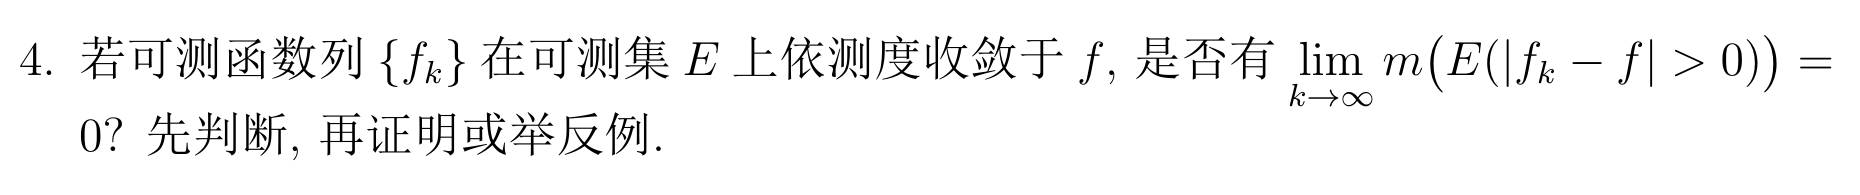
\includegraphics[width=\textwidth]{5-hw8-2025042920.png}
% \caption{}
\label{}
\end{figure}
\end{exercise}
$\lim_{ k \to \infty }m(E(\lvert f_k-f \rvert>0))=0$ 意味着几乎处处收敛,但依测度收敛并不蕴含几乎处处收敛.
\begin{figure}[H]
\centering
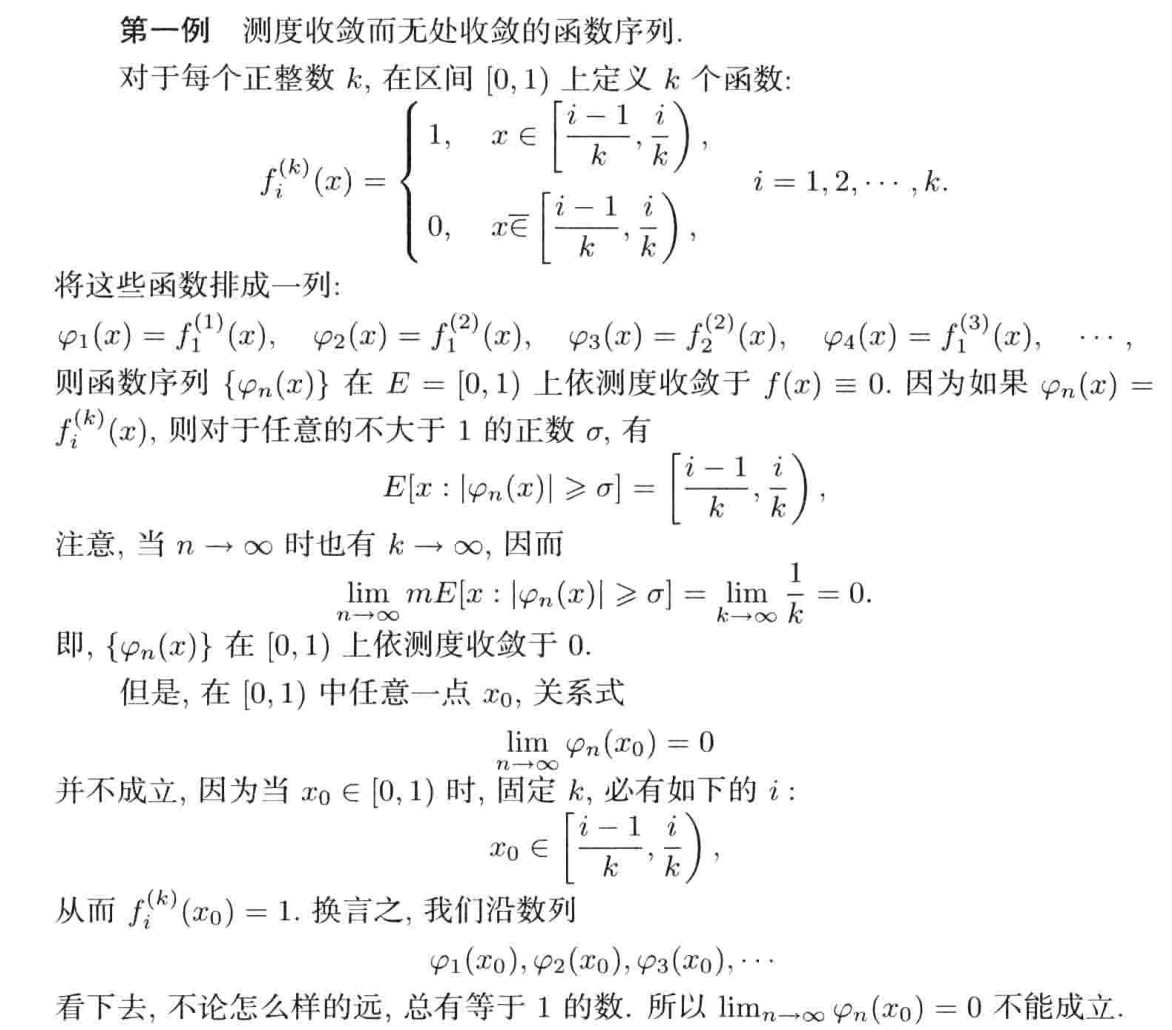
\includegraphics[width=\textwidth]{hw8-2025043009.png}
% \caption{}
\label{}
\end{figure}

\begin{exercise}
\begin{figure}[H]
\centering
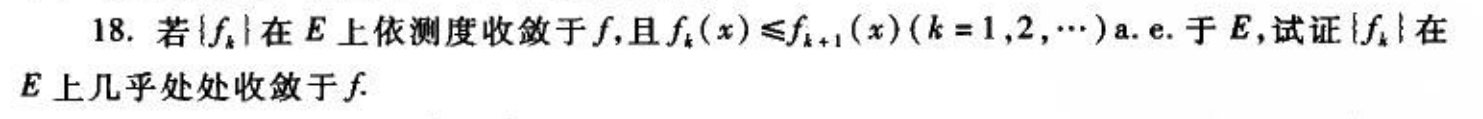
\includegraphics[width=\textwidth]{6-hw8-2025042920.png}
% \caption{}
\label{}
\end{figure}
\end{exercise}
由 Riesz 定理,存在 $\{ f_k \}$ 的子列 $\{ f_{k_i} \}$,使得 $\{ f_{k_i} \}$ 在 $E$ 上几乎处处收敛于 $f$. 也就是说
\[
\lim_{ i \to \infty } m(E(\lvert f_{k_i}-f \rvert >0))=0
\]
也就是对于任意给定的 $\epsilon>0$,存在 $N>0$, 使得对于任意 $i\geq N$,有
\[
m(E(\lvert f_{k_i}-f \rvert >0))<\epsilon \qquad
\]
由于 $f_k(x)\leq f_{k+1}(x)$, $k=1,2,\dots$ a.e. 于 $E$,我们有
\[
m(E(f_k>f_{k+1}))=0
\]
从而对于任意给定的 $k\in \{ 1,2,\dots \}$,
\[
m\left( \underbrace{ E(f<f_{k}) }_{ \subset \bigcup_{n=k}^{\infty} E(f_{n+1}<f_n) } \right)\leq \sum_{n=k}^{\infty} m(E(f_{n+1}>f_n))=0\implies m(E(f>f_k))=0
\]
从而
\[
m(E(f-f_{k}>0))=m(E(f-f_{k}>0))+m(E(f-f_{k}<0))=m(E(\lvert f-f_{k} \rvert >0))
\]
于是对于任意 $k>k_{N}$,我们有
\[
\begin{aligned}
m(E(\lvert f-f_{k} \rvert >0)) & =m\overbrace{ (E(f-f_k>0)  ) }^{ \subset E(f-f_{k_{N}}>0)\bigcup E(f_{k}-f_{k_{N}}>0) } \\
 & \leq m(E(f-f_{k_{N}}>0))+m(E(f_{k}-f_{k_{N}}>0)) \\
 & <\epsilon+0=\epsilon
\end{aligned}
\]
因此
\[
\lim_{ k \to \infty } m(E\lvert f-f_k \rvert >0)=0
\]
\begin{exercise}
\begin{figure}[H]
\centering
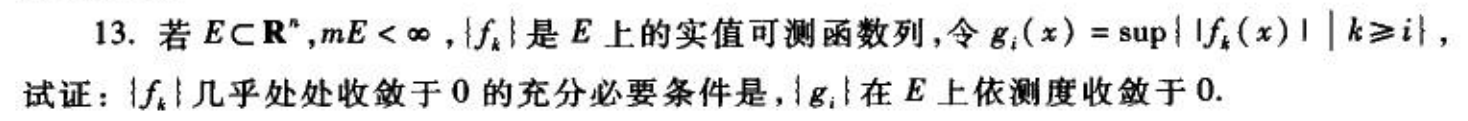
\includegraphics[width=\textwidth]{7-hw8-2025042920.png}
% \caption{}
\label{}
\end{figure}
\end{exercise}
\begin{proof}
By \cref{723813}, $\{ g_i \}\overset{ m }{ \to }0$ iff $\forall \{ g_{i_k} \}$, $\exists \{ g_{i_{k_j}} \}\to0$ a.e., that is, $\{ \sup_{n\geq i_{k_{j}}}\lvert f_n \rvert \}\to0$ a.e.

Suppose that $\{ g_i \}\overset{ m }{ \to }g$, then $\{ \sup_{n\geq i_{k_j}}\lvert f_n \rvert \}\to0$ a.e., i.e. for any $\epsilon>0$, there exists $N>0$ s.t.
\[
m(E(\sup_{n\geq i_{k_j}}\lvert f_n \rvert \neq 0))<\epsilon \qquad \forall j\geq N
\]
Then for any $n\geq i_{j_{N}}$, we have
\[
m(E(\lvert f_n \rvert \neq 0))\leq m\left( \bigcup_{n\geq i_{j_{N}}}^{} E(\lvert f_n \rvert \neq 0) \right)=m(E(\sup_{n\geq i_{j_{N}}}\lvert f_n \rvert \neq 0))<\epsilon
\]
Thus $f_n\to0$ a.e.

Suppose that $f_n\to0$ a.e. For any given $\{ g_{i_k} \}$, we have to find its subsequence $\{ g_{i_{k_j}} \}\to0$ a.e. There exists $Z$ with measure 0, s.t. $f_n\to0$ on $E\setminus Z$. There exists $i_{k_{j}}$ s.t. $\lvert f_n(x) \rvert\leq\frac{1}{j}$ on $E\setminus Z$, for any $n\geq i_{k_{j}}$. Thus
\[
g_{i_{k_{j}}}(x)=\sup_{n\geq i_{k_{j}}}\lvert f_n(x) \rvert \leq \frac{1}{j}\to0\qquad \text{as }j\to \infty
\]
Thus $g_{i_{k_j}}\to0$ as $j\to \infty$ on $E\setminus Z$, i.e. $g_{i_{k_j}}\to0$ a.e. Then we are done!
\end{proof}

\begin{exercise}
\begin{figure}[H]
\centering
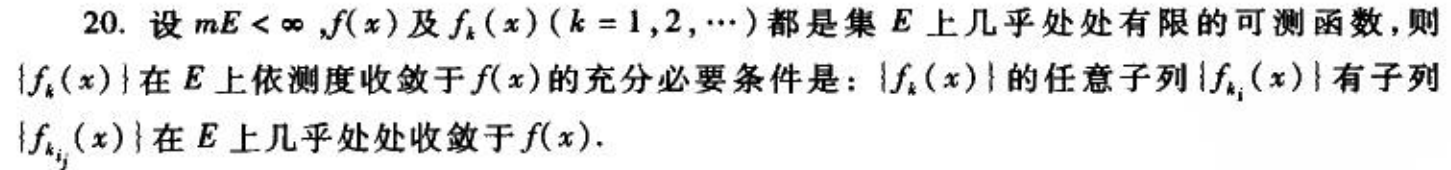
\includegraphics[width=\textwidth]{8-hw8-2025042920.png}
% \caption{}
\label{}
\end{figure}\label{723813}
\end{exercise}

\begin{proof}
若 $f_k\overset{ m }{ \to }f$,则 $f_{k_i}\overset{ m }{ \to }f$,由 Riesz 定理,存在 $\{ f_{k_{i_j}} \}\to f$ a.e.

若 $\forall \{ f_{k_i} \}$, $\exists \{ f_{k_{i_{j}}}(x) \}\to f(x)$ a.e. 假设 $f_k \overset{ m }{ \not\to }f$,也就是存在 $\eta_0>0$,使得
\[
a_k\coloneqq m(E(\lvert f_k-f \rvert >\eta_0))\not\to0
\]
于是 $\{ a_k \}$ 存在子列 $\{ a_{k_i} \}\to c>0$, 其中 $c\in \overline{\mathbb{R}}$. 又由于 $\{ f_{k_{i_j}}(x) \}\to f(x)$ a.e. 那么 $a_{k_{i_j}}\to0$,但是
\[
0=\lim_{ i \to \infty } a_{k_i}=\lim_{ j \to \infty } a_{k_{i_j}}=c>0
\]
矛盾!
\end{proof}

\begin{exercise}
\begin{figure}[H]
\centering
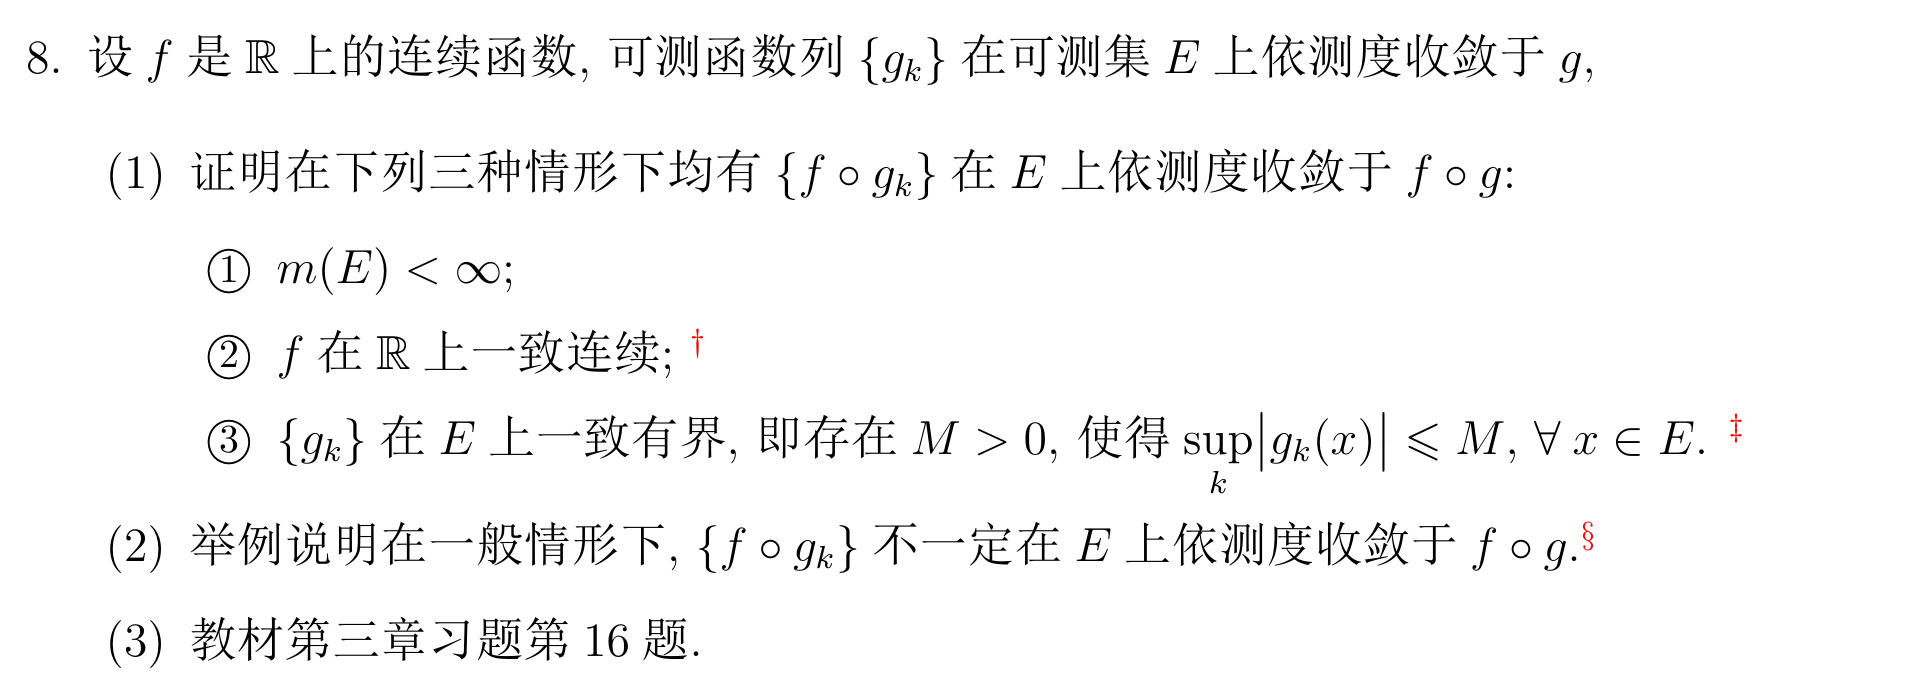
\includegraphics[width=\textwidth]{9-hw8-2025042920.png}
% \caption{}
\label{}
\end{figure}
\begin{figure}[H]
\centering
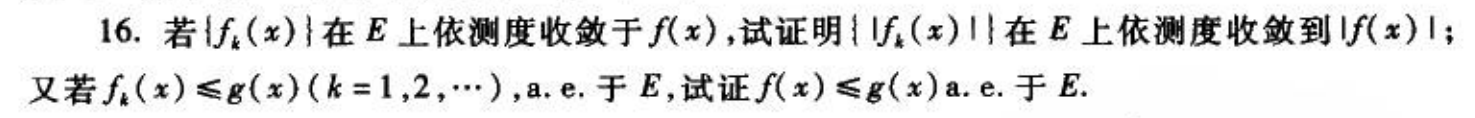
\includegraphics[width=\textwidth]{10-hw8-2025042920.png}
% \caption{}
\label{}
\end{figure}
\end{exercise}
(1)
If $mE<\infty$, then for any $\{ f \circ g_{k_i} \}$, by Riesz's theorem, $\exists \{ g_{k_{i_j}} \}\to g$ a.e. That is, $\exists Z$ with measure 0, s.t. $g_{k_{i_j}}\to g$ on $E\setminus Z$. Since $g$ is continuous, we have $f\circ g_{k_{i_j}}\to f\circ g$ on $E\setminus Z$. Thus $f\circ g_{k_{i_j}}\to f\circ g$ a.e. By \cref{723813} we are done.

If $f$ is uniformly continuous on $\mathbb{R}$, then $\forall\epsilon>0$, $\exists\delta>0$, s.t.
\[
\lvert f(x)-f(y) \rvert <\epsilon \qquad \forall \lvert x-y \rvert <\delta
\]
which means $\lvert x-y \rvert<\delta$ implies $\lvert f(x)-f(y) \rvert<\epsilon$ and $\lvert x-y \rvert\geq\delta$ implies $\lvert f(x)-f(y) \rvert\geq\epsilon$. Since $g_{k}\overset{ m }{ \to }g$, we also have $m(E(\lvert g_k-g\rvert>\delta))\to0$, as $k\to \infty$. Then
\[
\begin{aligned}
m(E(\lvert f\circ g_k-f\circ g \rvert >\epsilon)) & =m\{ x\in E:\lvert f(g_k(x))-f(g(x)) \rvert >\epsilon \} \\
 & \leq m\{ x\in E:\lvert g_k(x)-g(x) \rvert >\delta  \} \\
 & =m(E(\lvert g_k-g \rvert >\epsilon))\to0\qquad \text{as }k\to \infty 
\end{aligned}
\]
If $\{ g_k \}$ is uniformly bounded on $E$, i.e. $\exists M>0$, s.t. $\sup_{k}\lvert g_k(x) \rvert\leq M$, $\forall x\in E$. We restrict $f$ to $[-M-1,M+1]$, then $f\circ g_k=\left.f\right|_{[-M-1,M+1]}\circ g_k$, and $f$ is uniformly continuous on the closed interval $[-M-1,M+1]$. Apply (2), we have $f\circ g_k\overset{ m }{ \to } \left.f\right|_{[-M-1,M+1]}\circ g$. For any $1>\epsilon>0$,
\[
\begin{aligned}
m(E(\lvert f\circ g_k-f\circ g \rvert >\epsilon)) & =m(E(\lvert f\circ g_k-f\circ g \rvert >\epsilon)\cap \{ x\in E:\lvert g(x)\rvert \leq M+1 \}) \\
 & \quad +m(E(\lvert f\circ g_k-f\circ g \rvert >\epsilon)\cap \{ x\in E:\lvert g(x) \rvert >M+1 \}) \\
 & \leq m(E(\lvert f\circ g_k-f\circ g \rvert >\epsilon)\cap \{ x\in E:\lvert g(x)\rvert \leq M+1 \}) \\
 & \quad +m\{ x\in E:\lvert g(x) \rvert >M+1 \}  \\
 & \leq m(E(\lvert f\circ g_k-f\circ g \rvert >\epsilon)\cap \{ x\in E:\lvert g(x)\rvert \leq M+1 \}) \\
 & \quad +m(E(\lvert g-g_k \rvert >\epsilon))   \\
 & \to0\qquad \text{as }k\to \infty
\end{aligned}
\]
(2)

(3)
Since $f_k\overset{ m }{ \to }f$ then $\forall\epsilon>0$, $m(E(\lvert f_k-f \rvert>\epsilon))\to0$ as $k\to \infty$. Due to the inequality,
\[
\lvert f_k-f \rvert \geq \lvert \lvert f_k \rvert -\lvert f \rvert  \rvert
\]
We have the inclusion of sets.
\[
E(\lvert f_k-f \rvert >\epsilon)\supseteq E(\lvert \lvert f_k \rvert -\lvert f \rvert  \rvert >\epsilon)
\]
Thus
\[
m(E(\lvert \lvert f_k \rvert -\lvert f \rvert  \rvert >\epsilon))\leq m(E(\lvert f_k-f \rvert >\epsilon))
\]
Let $k\to \infty$, then $m(E(\lvert \lvert f_k \rvert-\lvert f \rvert \rvert>\epsilon))\to0$. Hence $\lvert f_k \rvert\overset{ m }{ \to }\lvert f \rvert$.

By Riesz's theorem, there exists a subsequence $\{ f_{k_i} \}\to f$ a.e. Since $f_k(x)\leq g(x)$ a.e. on $E$, we have
\[
\lim_{ k \to \infty } m(E(f_k>g))=0\qquad \text{and}\qquad \lim_{ i \to \infty } m(E(f_{k_i}\neq f))=0
\]
Then
\[
\begin{aligned}
E(f>g) & =[E(f>g)\cap E(f_{k_i}\neq f)]\cup[E(f>g)\cap E(f_{k_i}=f)] \\
 & \subset E(f_{k_i}\neq f)\cup E(f_{k_i}>g)
\end{aligned}
\]
Therefore
\[
m(E(f>g))\leq m(E(f_{k_i}\neq f))+m(E(f_{k_i}>g))\to0\qquad \text{as }k,i\to \infty
\]
Hence $f<g$ a.e. on $E$.

\begin{exercise}
\begin{figure}[H]
\centering
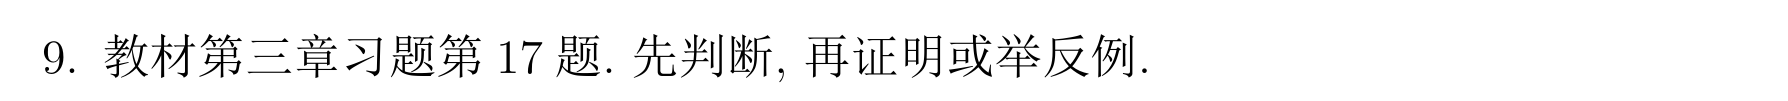
\includegraphics[width=\textwidth]{11-hw8-2025042920.png}
% \caption{}
\label{}
\end{figure}
\begin{figure}[H]
\centering
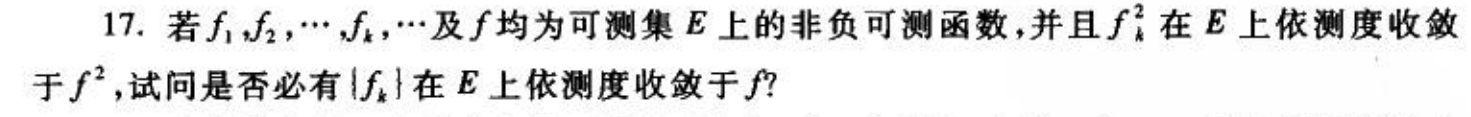
\includegraphics[width=\textwidth]{12-hw8-2025042920.png}
% \caption{}
\label{}
\end{figure}
\end{exercise}
并不一定.

\begin{exercise}
\begin{figure}[H]
\centering
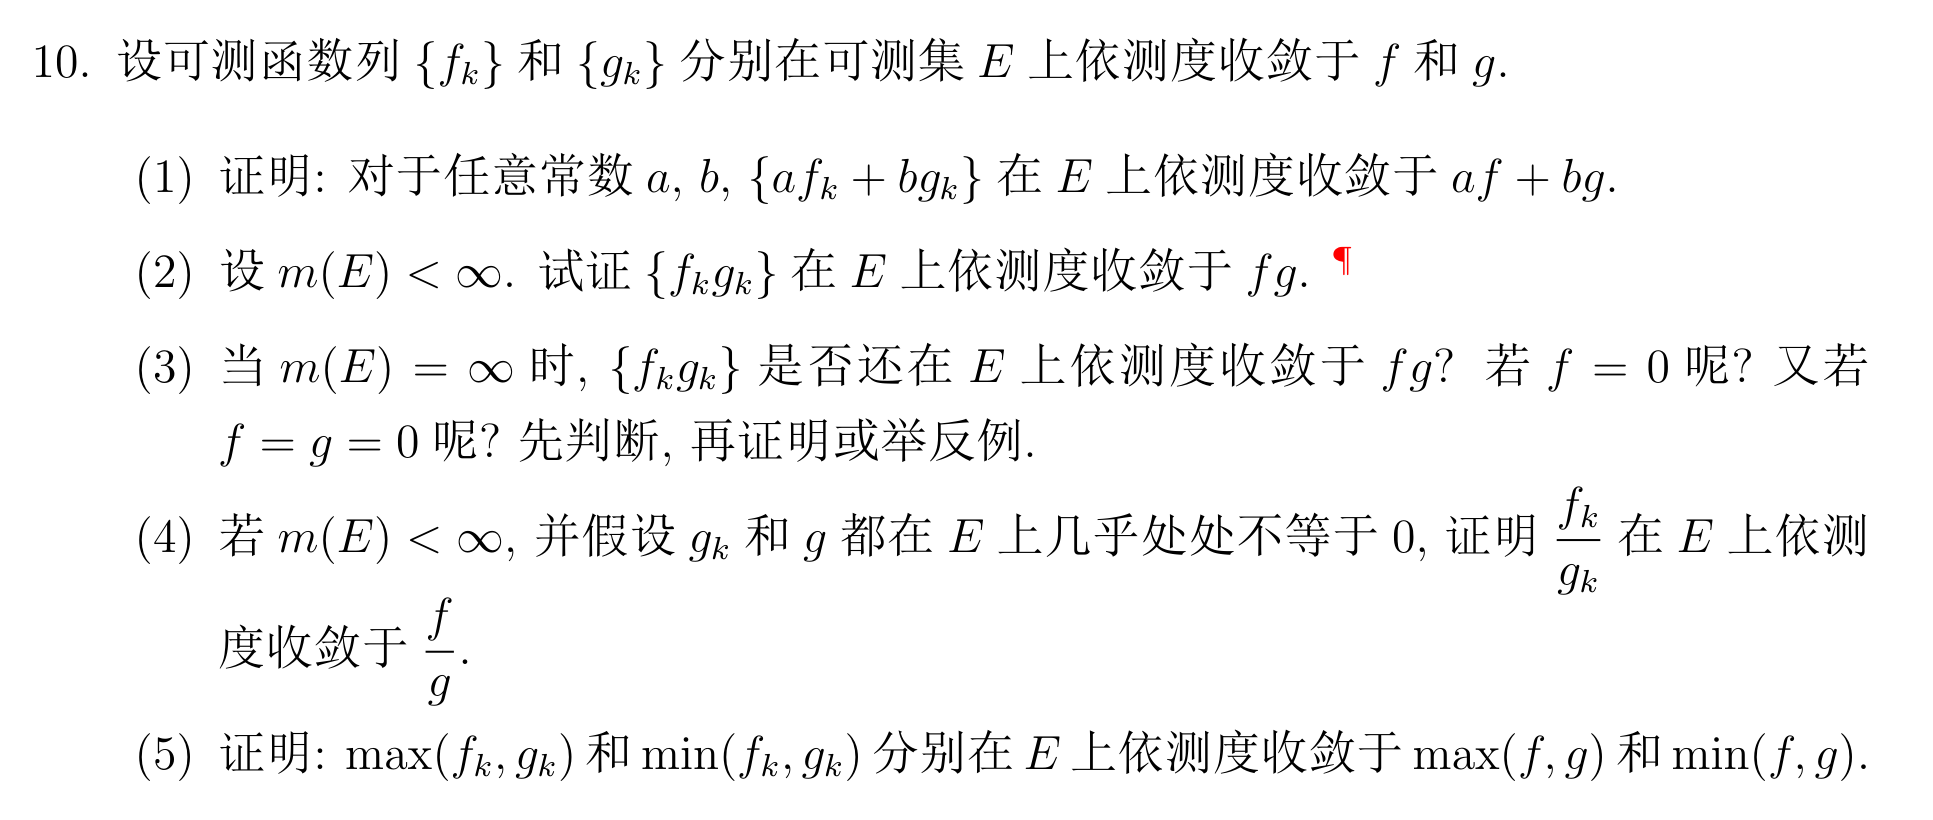
\includegraphics[width=\textwidth]{13-hw8-2025042920.png}
% \caption{}
\label{}
\end{figure}
\end{exercise}
(1) 若 $a,b$ 有一者为零,则显然. 若 $a,b$ 非零,则
\[
\begin{aligned}
m(E(\lvert af_k+bg_k -af-bg\rvert >\epsilon)) & \leq m\left( E\left( \lvert f_k-f \rvert >\frac{\epsilon}{\lvert a \rvert } \right)\cup E\left( \lvert g_k -g\rvert >\frac{\epsilon}{\lvert b \rvert } \right) \right) \\
 & \leq m\left( E\left( \lvert f_k-f \rvert >\frac{\epsilon}{\lvert a \rvert } \right) \right)+m\left( E\left( \lvert g_k -g\rvert>\frac{\epsilon}{\lvert b \rvert }  \right) \right) \\
 & \to0\qquad (\text{as }k\to \infty)
\end{aligned}
\]
(2)
利用 Riesz 定理,我们有对于任意 $\{ f_{k_i}g_{k_i} \}$,存在 $f_{k_{i_j}}\to f$ a.e.,存在 $g_{k_{i_{j_{l}}}}\to g$ a.e. 从而 $f_{k_{i_{j_{l}}}}g_{k_{i_{j_{l}}}}\to fg$ a.e. 再利用  \cref{723813} 可知 $f_kg_k\overset{ m }{ \to }fg$.

(3)
$mE=\infty$ 时存在反例.
\begin{figure}[H]
\centering
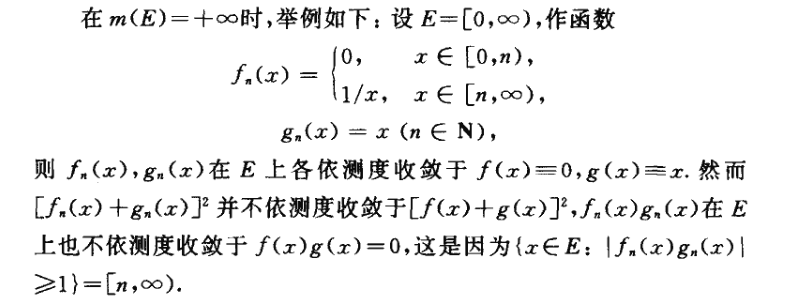
\includegraphics[width=\textwidth]{1-hw8-2025043012.png}
% \caption{}
\label{}
\end{figure}
$f=0$ 时存在反例,但 $f=g=0$ 时结论成立,证明如下
\[
m(E(\lvert f_kg_k \rvert >\epsilon))\leq m(E(\lvert f_k \rvert >\sqrt{ \epsilon }))+m(E(\lvert g_k \rvert >\sqrt{ \epsilon }))\to0\quad (\text{as }k\to \infty)
\]
(4)
利用 Riesz 定理,我们有对于任意 $\left\{  \frac{f_{k_i}}{g_{k_i}}  \right\}$,存在 $f_{k_{i_j}}\to f$ a.e.,存在 $g_{k_{i_{j_{l}}}}\to g$ a.e. 从而 $\frac{f_{k_{i_{j_{l}}}}}{g_{k_{i_{j_{l}}}}}\to \frac{f}{g}$ a.e. 再利用  \cref{723813} 可知 $\frac{f_k}{g_k}\overset{ m }{ \to }\frac{f}{g}$.

(5)
\[
\max(f_k,g_k)=f_k+g_k+\lvert f_k-g_k \rvert,\qquad \min(f_k,g_k)=f_k+g_k-\lvert f_k-g_k \rvert
\]
断言:$\lvert f_k-g_k \rvert\overset{ m }{ \to }\lvert f-g \rvert$,这是因为
\[
\begin{aligned}
m(E(\lvert \lvert f_k-g_k \rvert -\lvert f-g \rvert  \rvert >\epsilon)) & \leq m(E(\lvert f_k-f \rvert +\lvert g_k-g \rvert >\epsilon)) \\
 & \leq m(E(\lvert f_k-f \rvert >\epsilon)\cup E(\lvert g_k-g \rvert >\epsilon) ) \\
 & \leq m(E(\lvert f_k-f \rvert >\epsilon))+m(E(\lvert g_k-g \rvert >\epsilon)) \\
 & \to0\qquad (\text{as }k\to \infty)
\end{aligned}
\]
再结合 (1) 可知,$\max(f_k,g_k)\overset{ m }{ \to }\max(f,g)$, $\min(f_k,g_k)\overset{ m }{ \to }\min(f,g)$.
